\documentclass[11pt]{article}
\usepackage[margin=1in]{geometry}
\usepackage{graphicx}
\usepackage{amsmath}
\usepackage{booktabs}
\usepackage{hyperref}
\usepackage{caption}
\usepackage{microtype}
\usepackage[numbers,sort&compress]{natbib}

% Helvetica everywhere (sans-serif body + math)
\usepackage[T1]{fontenc}
\usepackage[scaled]{helvet}
\renewcommand{\familydefault}{\sfdefault}

\usepackage{xcolor}
\hypersetup{colorlinks=true, linkcolor=blue!50!black,
            citecolor=blue!50!black, urlcolor=blue!50!black}

\title{Alignment, position-based, and hybrid models of locust collective
motion: a four-metric calibration against field trajectories}

\author{Asher Albrecht \and George Stephenson \\
Department of Computer Science, University of Colorado Boulder}

\date{CSCI-5423: Biologically Inspired Multi-Agent Systems \\ Spring 2026}

\begin{document}
\maketitle

\begin{abstract}
We test which local interaction rule reproduces the collective motion of
free-ranging locust hopper bands. We simulate the Vicsek alignment model
\citep{vicsek1995}, a position-based pull model after \citet{sayin2025},
and a sequence of hybrids that combine forward-weighted alignment,
anisotropic noise, heading inertia, and a soft preferred-spacing zone. We
compare each model to the trajectory dataset of \citet{weinburd2024}
across four metrics: polarization $\Phi$, turning-angle standard deviation,
nearest-neighbor distance, and a global anisotropy index of the
body-centered neighbor density. The two baseline models fail in distinct,
mechanistic ways. Hand-tuning a hybrid closed some gaps but introduced
others. We replace hand-tuning with the Covariance Matrix Adaptation
Evolution Strategy (CMA-ES) \citep{hansen2016}, parallelized across 24
CPU cores, and search a six- and seven-dimensional parameter space against
a weighted relative-error loss. The calibrated six-parameter hybrid (v4)
matches all three scalar field metrics within 10\% and reproduces the
field's body-centered neighbor density both globally
($A_\text{global} \approx 0$) and inside a 1.5--3.0\,cm near-zone band
($A_\text{near} = -0.005$ for both v4 and the field). A
seven-parameter variant adding temporal bearing integration (v5)
reaches a marginally lower scalar loss but lands in a different basin
where the preferred-spacing ring carries a forward-bias artifact
($A_\text{near} = -0.06$) that the field does not have; the seventh
parameter is unnecessary at the field's measurement scale and worsens
the spatial fit. The fit depends on periodic boundaries; under
reflective walls the calibration breaks, which we discuss as a
limitation for any claim about open hopper-band geometry.
\end{abstract}

\section{Introduction}

Australian plague locusts (\textit{Chortoicetes terminifera}) form
hopper bands that march coherently across kilometers of terrain, causing
agricultural damage at continental scale. Two competing theories of how
they coordinate have appeared in the literature. The first, originating
with \citet{vicsek1995} and applied to locusts by \citet{buhl2006},
proposes that each individual aligns its heading with neighbors inside a
fixed radius. Order arises from a density-driven phase transition. The
second, advocated by \citet{sayin2025}, proposes that individuals are
attracted to the positions of forward neighbors. The interaction is
geometric rather than directional, and order is a byproduct of position
tracking rather than heading averaging.

These theories make different predictions about the spatial structure of
the swarm and about the frame-to-frame heading dynamics of individuals.
Until recently they could not be tested against individual-level field
data. \citet{weinburd2024} released the first such dataset: roughly 3.3
million position records and 20{,}000 trajectories from four hopper bands,
sampled at 25\,Hz. We use this dataset as the ground truth.

We ask which local rule, or which combination of rules, reproduces the
field measurements. Our contribution is twofold. First, we show that
both pure alignment and pure pull fail in characteristic ways and that a
hand-tuned hybrid trades one failure for another. Second, we replace
hand-tuning with derivative-free optimization: CMA-ES searches the
parameter space against a multi-metric loss and finds a hybrid that fits
the field on every metric we tested. The methodological pivot, from
exploring a few parameter combinations to optimizing many jointly, is the
main lesson of the work.

\section{Background and related work}

The Vicsek model \citep{vicsek1995} is a minimal self-propelled particle
system: at each time step, every agent updates its heading to the
arithmetic mean of neighbor headings inside an interaction radius, plus
uniform angular noise of width $\eta$. \citet{buhl2006} fit this model to
laboratory locust experiments and reported a phase transition from
disorder to coherent marching as density increased. \citet{bazazi2008}
proposed an alternative mechanism in which collisions and cannibalism
drive forward motion. Neither study had access to free-ranging field
trajectories.

\citet{weinburd2024} computed body-centered neighbor density maps from
their hopper-band data and observed an asymmetric distribution: more
density behind the focal individual than ahead, with the dominant signal
in the near zone. They argued for directional interactions but stopped
short of a specific mechanistic model.

\citet{sayin2025} fit a position-based model to laboratory and modeling
experiments. In their pull formulation, each agent steers toward a
weighted centroid of forward neighbors, with weights proportional to
$\cos^2(\beta/2)$ for relative bearing $\beta$. They argued that this
mechanism can produce coherent motion without explicit alignment.

The Couzin model \citep{couzin2002} combines repulsion, alignment, and
attraction in nested zones. We borrow the soft preferred-spacing idea
from this literature for our hybrid extensions.

CMA-ES \citep{hansen2016} is a derivative-free evolutionary optimizer
that adapts a multivariate Gaussian sampling distribution as it explores.
It is well suited to noisy black-box objectives in low-dimensional
continuous spaces. We use the \texttt{pycma} implementation
\citep{pycma}.

\section{Methods}

\subsection{Field metrics}

We compute four metrics from the Weinburd dataset and apply the same
functions to every simulated trajectory:

\begin{enumerate}
\item Global polarization $\Phi(t) = \left| \frac{1}{N(t)} \sum_i
  e^{i\theta_i(t)} \right|$, averaged over time after burn-in.
\item Turning-angle standard deviation: per-step heading change
  $\Delta\theta_i(t) = \theta_i(t+1) - \theta_i(t)$, wrapped to
  $[-\pi, \pi]$, pooled across agents and time.
\item Median nearest-neighbor distance (NND).
\item Body-centered neighbor density. For each focal individual we
  rotate the relative position of every neighbor inside a 10\,cm radius
  into the focal's body frame (heading along $+y$) and accumulate a
  $50 \times 50$ histogram. Figure~\ref{fig:fig1} shows the field
  distribution.
\end{enumerate}

From the density map we derive a scalar global anisotropy index
$A = (\rho_\text{rear} - \rho_\text{front}) / (\rho_\text{rear} +
\rho_\text{front})$, where $\rho_\text{rear}$ and $\rho_\text{front}$ are
the mean densities in the lower and upper halves of the body-centered
histogram. $A > 0$ indicates more density behind the focal than ahead.

\begin{figure}[t]
\centering
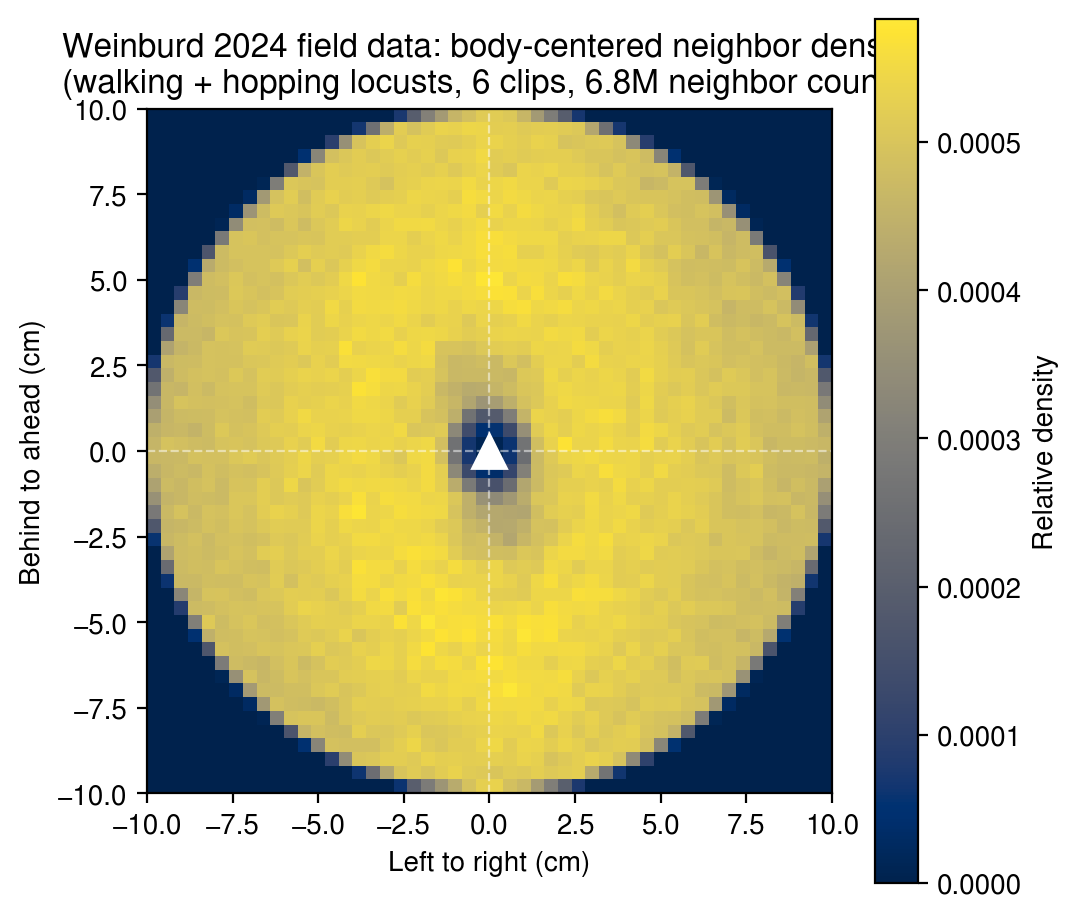
\includegraphics[width=0.55\linewidth]{figures/fig1_field_density.png}
\caption{Body-centered neighbor density from the Weinburd 2024 hopper-band
dataset, walking and hopping individuals combined (six clips,
$6.86 \times 10^6$ neighbor counts). The focal heads up. The distribution
is close to isotropic at the global level ($A_\text{field} = -0.0008$),
with a self-exclusion hole at the origin. We use this map and its scalar
summary as a fourth field-fitting target alongside the three scalar
metrics.}
\label{fig:fig1}
\end{figure}

\subsection{Models}

The Vicsek model implements standard alignment dynamics with periodic
boundaries. Each agent sets its next heading to
$\theta_i(t{+}1) = \arg\!\sum_{j \in \mathcal{N}_i}
e^{i\theta_j} + \eta \xi_i$, where $\mathcal{N}_i$ is the set of
neighbors within $r_\text{int} = 7\,$cm and $\xi_i \sim
\mathcal{U}(-1/2, 1/2)$. Speed is constant and a hard repulsion override
applies at $r_\text{rep} = 1.5\,$cm.

The pull model has each agent steer toward the centroid of forward
neighbors weighted by $w(\beta) = \cos^2(\beta/2)$, following
\citet{sayin2025}. The noise term and the repulsion override match the
Vicsek implementation.

Hybrid v3 (anisotropic Vicsek) extends the alignment rule along two
axes. Forward neighbors (relative bearing $|\beta| < \pi/3$) get
weight $1 + \alpha_\text{aniso}$ and rear neighbors $1 -
\alpha_\text{aniso}$. Effective noise scales with the fraction of
neighbors ahead: $\eta_\text{eff}(i) = \eta_\text{base} (1 - \lambda
f_\text{forward}(i))$. Speed varies with local order between
$v_\text{min}$ and $v_\text{max}$.

Hybrid v4 adds two mechanisms motivated by the v3 failure analysis
(Section~\ref{sec:results}). The heading-inertia term has each agent
commit a fraction $\mu \in (0, 1]$ of the way to its new desired
heading $\theta^*$ via exponential smoothing in unit-vector space:
$\theta_{i}(t{+}1) = \arg\!\left[(1{-}\mu) e^{i\theta_i(t)} + \mu
e^{i\theta^*}\right]$. This narrows the per-step turning distribution.
The preferred-spacing zone applies in the band $r_\text{rep} < d <
r_\text{pref}$: the agent mixes a radial-push direction into its
desired heading with weight $k_\text{pref}$.

Hybrid v5 adds temporal bearing integration after \citet{sayin2025}'s
ring-attractor analogy. Each agent maintains an exponential moving
average of the alignment-derived target unit vector, $T_\text{ema}
\leftarrow (1-\rho) T_\text{ema} + \rho T_\text{instantaneous}$. The
desired heading derives from $T_\text{ema}$ rather than the
instantaneous target. Setting $\rho = 1$ disables the integrator and
recovers v4.

\subsection{Calibration}

We calibrate the hybrid models with CMA-ES against a weighted relative-error
loss
\begin{align}
L = w_\Phi \frac{|\Phi_\text{sim} - \Phi_\text{field}|}{\Phi_\text{field}}
  + w_\sigma \frac{|\sigma_\text{sim} - \sigma_\text{field}|}{\sigma_\text{field}}
  + w_\text{NND} \frac{|\text{NND}_\text{sim} - \text{NND}_\text{field}|}{\text{NND}_\text{field}},
\end{align}
with weights $w_\Phi = 1$, $w_\sigma = w_\text{NND} = 2$. The two
failure-mode metrics from the baseline experiments (Section~\ref{sec:results})
get double weight; polarization is already close in v3. Each evaluation
runs five seeds of a 2000-step simulation with 500-step burn-in and
returns the ensemble mean.

The optimization parameter space is six-dimensional for v4 and
seven-dimensional for v5: $\eta_\text{base} \in [0.1, 1.5]$,
$\lambda \in [0, 1]$, $\alpha_\text{aniso} \in [0, 1]$,
$\mu \in [0.1, 1.0]$, $k_\text{pref} \in [0, 0.7]$,
$r_\text{pref} \in [1.6, 5.0]$\,cm, and (v5 only)
$\rho_\text{temporal} \in [0.05, 1.0]$. Following the \texttt{pycma}
guidance \citep{pycma}, we map every parameter linearly to the internal
range $[0, 10]$ so a single $\sigma_0$ has uniform meaning across
dimensions.

We run CMA-ES with population size 20, $\sigma_0 = 2.0$, and 40--50
generations. The 20 candidate evaluations within each generation are
distributed across CPU cores using \texttt{multiprocessing.Pool}; BLAS
threading inside workers is pinned to one to avoid oversubscription. On
a 32-thread Intel i9-13900K the full v4 optimization completes in
about 13 minutes (gen$_0$ in 19 seconds, end-to-end speedup of about
$11{\times}$ over the serial implementation).

\section{Results}
\label{sec:results}

\subsection{The two baselines fail in distinct ways}

After calibrating $\eta$ to match field polarization, the Vicsek model
hits $\Phi = 0.82$ (target 0.820) but produces a turning-angle
distribution more than twice as wide as the field
(0.595\,rad vs 0.276\,rad, 116\% relative error) and undercounts NND by
33\%. The model achieves order, but at the cost of pathological
heading noise that compensates for the absence of any heading-stabilizing
mechanism beyond raw alignment.

The pull model fails differently. Across five structural variants we
tested (varying cone half-angle, pull strength, and noise), polarization
remained at $\Phi \approx 0.06$, with a turning-angle distribution near
$2\,$rad (essentially saturated). The geometric reason is that, in a
disordered swarm, neighbor bearings are uniformly distributed around the
focal, and the forward-weighting function $\cos^2(\beta/2)$ is symmetric
under reflection. The expected pull direction is along the focal
heading, with no symmetry breaking that would amplify small alignment
fluctuations into global order.

Hybrid v3 (anisotropic Vicsek with hand-tuned $\eta = 1.1$, $\lambda =
0.8$, $\alpha = 0.6$) hits polarization within 0.5\% but still misses
turning-angle std by 215\% and NND by 55\%. Forward weighting tightens
the alignment, which lowers $\eta$ enough to bring polarization in at a
sensible noise level, but introduces no mechanism that limits per-step
heading change or sets a preferred spacing.

\subsection{CMA-ES closes the scalar gaps}
\label{sec:cma-closes}

\begin{figure}[t]
\centering
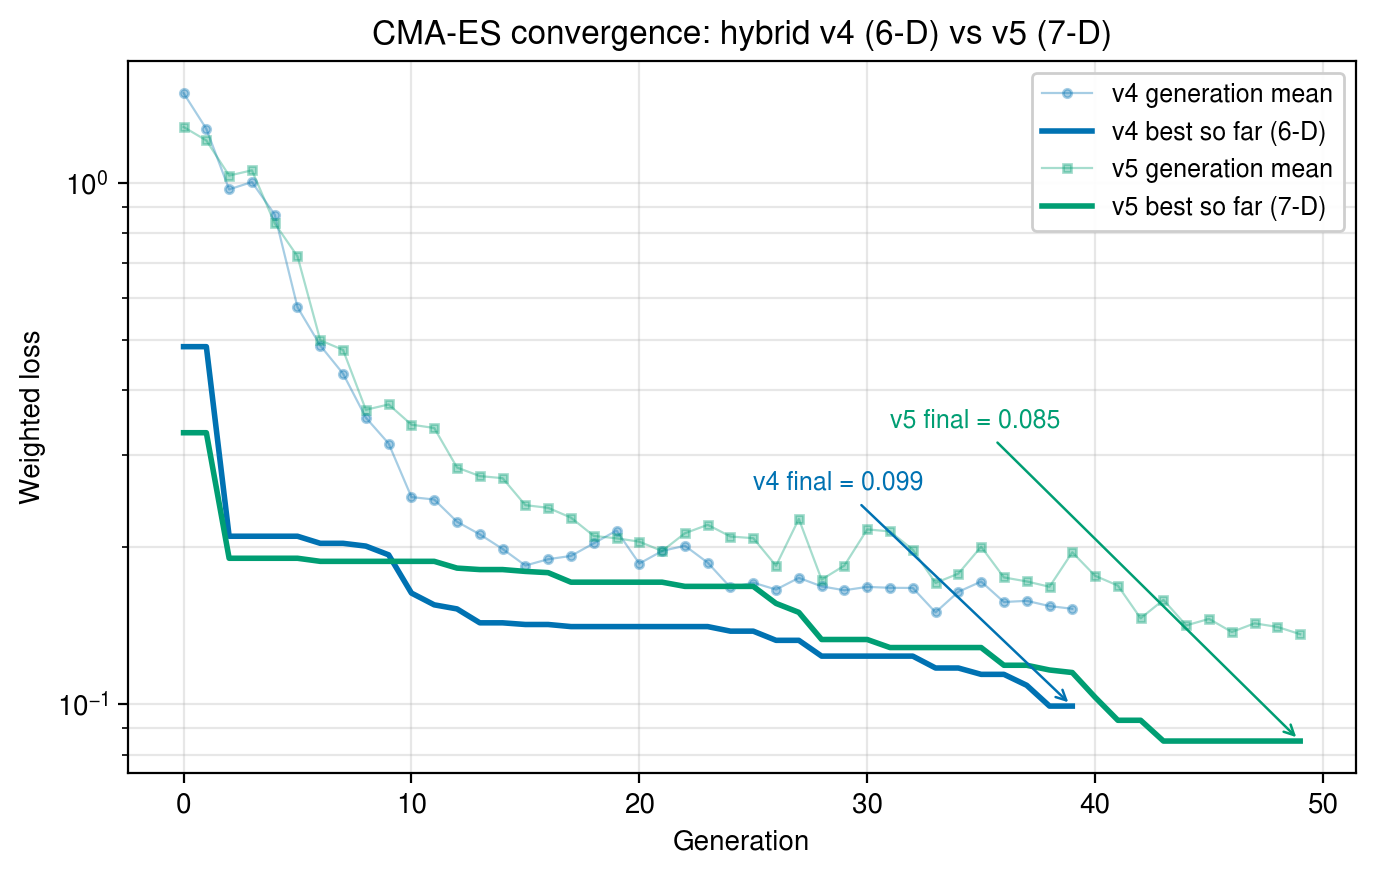
\includegraphics[width=0.85\linewidth]{figures/fig2_cma_convergence.png}
\caption{CMA-ES convergence curves. Both v4 (six-dimensional) and v5
(seven-dimensional) reduce the weighted loss by an order of magnitude over
40--50 generations. The v5 run plateaus around generation 25 before a late
breakout finds a slightly better basin.}
\label{fig:fig2}
\end{figure}

Figure~\ref{fig:fig2} shows the loss trajectories. The v4 run reaches a
final loss of 0.099, with $\Phi = 0.898$ (9.6\% off the field),
turning-angle std $= 0.276$\,rad (0.001\% off), and NND median $=
3.899$\,cm (0.2\% off). The two failure modes that motivated heading
inertia and preferred spacing close to within seed noise. Polarization
remains slightly elevated.

The v5 run reaches 0.085, but the converged $\rho_\text{temporal} = 0.95$
is at the no-effect end of its allowed range. The improvement comes from
the optimizer escaping a 6-D local minimum into a different basin, not
from using the new mechanism. Specifically, $\alpha_\text{aniso}$ saturates at
1.0 and $\lambda$ drops to 0.17, while the other parameters move only
slightly. The basin v5 escaped into is worse on the spatial metric we
introduce in Section~\ref{sec:spatial}, so the marginally lower scalar
loss does not generalize.

Figure~\ref{fig:fig3} summarizes per-metric performance for every model
we ran. Numerical values are listed in Table~\ref{tab:scorecard}. The
two CMA-ES-calibrated runs separate further once the spatial structure
is examined directly (Section~\ref{sec:spatial}): v4 reproduces the
field's near-zone density, v5 does not.

\begin{figure}[t]
\centering
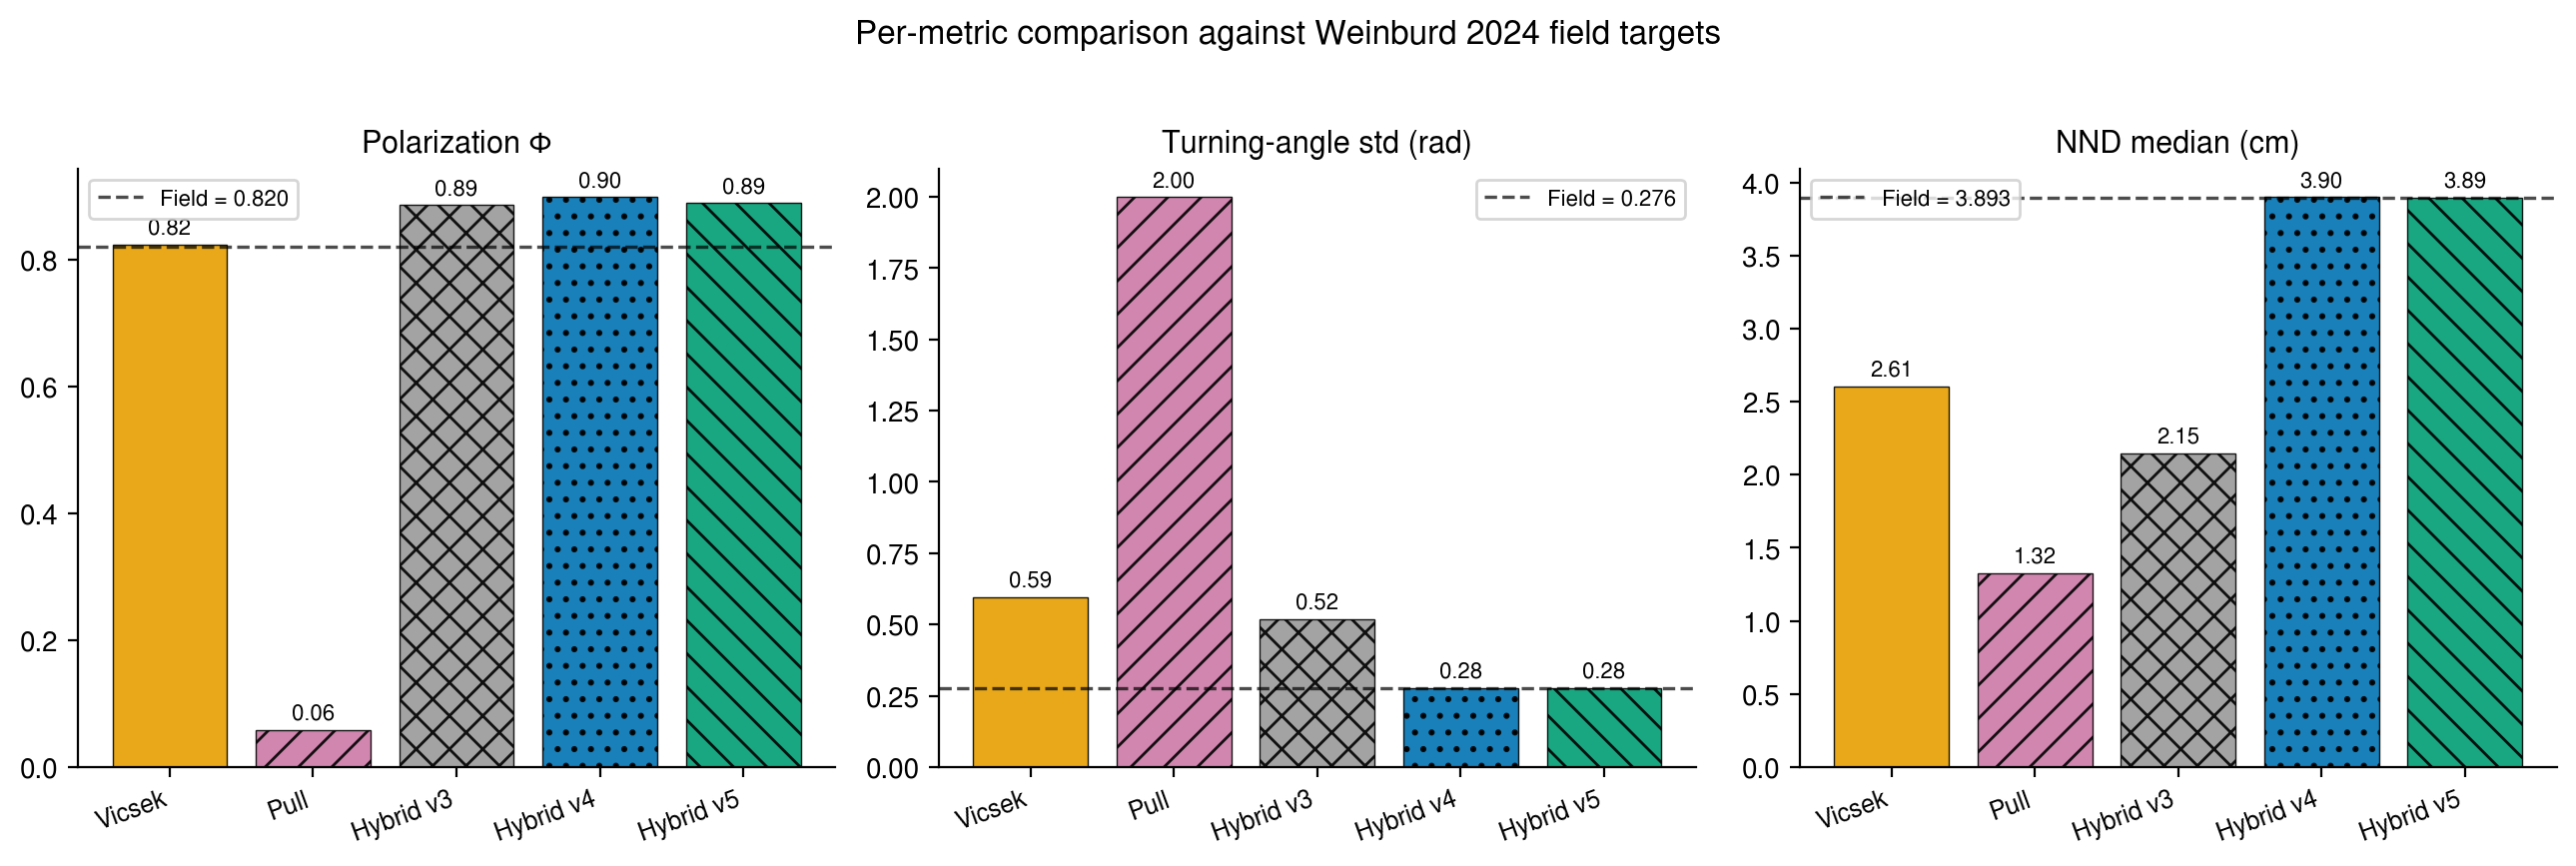
\includegraphics[width=\linewidth]{figures/fig3_scorecard.png}
\caption{Field-fit scorecard across all models on the three scalar
metrics. Dashed lines indicate field targets. Vicsek and Pull miss
multiple metrics. Hybrid v3 closes polarization but not the others.
CMA-ES-calibrated v4 and v5 hit all three scalar targets within seed
noise. The body-centered spatial structure separates v4 from v5; see
Figure~\ref{fig:fig4}.}
\label{fig:fig3}
\end{figure}

\begin{table}[t]
\centering
\small
\caption{Field-fit scorecard. Relative error in parentheses. Field targets:
$\Phi = 0.820$, $\sigma = 0.276$\,rad, NND $= 3.893$\,cm.
$\pm$ values on $\Phi$ are the across-seed standard deviation of the
per-seed mean (10 seeds for the baseline runs, 5 seeds for the
CMA-ES-calibrated runs).}
\label{tab:scorecard}
\begin{tabular}{lrrr}
\toprule
Model       & $\Phi$ \;$\pm\,\sigma_\text{seed}$       & $\sigma$ (rad)     & NND (cm)              \\
\midrule
Vicsek      & $0.824 \pm 0.019$ \;(0.5\%)              & 0.595 (116\%)      & 2.61 (33\%)           \\
Pull        & $0.058 \pm 0.001$ \;(93\%)               & 1.999 (624\%)      & 1.32 (66\%)           \\
Hybrid v3   & $0.890 \pm 0.025$ \;(8.5\%)              & 0.520 (88\%)       & 2.15 (45\%)           \\
Hybrid v4   & $0.898 \pm 0.027$ \;(9.6\%)              & 0.276 (0.001\%)    & 3.90 (0.2\%)          \\
Hybrid v5   & $0.889 \pm 0.012$ \;(8.4\%)              & 0.276 (0.05\%)     & 3.89 (0.04\%)         \\
\bottomrule
\end{tabular}
\end{table}

\subsection{Spatial structure: v4 matches, v5 distorts}
\label{sec:spatial}

The body-centered neighbor density map is the test that motivated the
hybrid in the first place. \citet{weinburd2024} reported anisotropic
neighbor distributions in their data, and our hybrid v3 reproduced a
visible asymmetry in the inner ring of its density map.

The global anisotropy index is essentially zero in the field
($A_\text{global} = -0.0008$). v3, v4, and v5 all reproduce the
global value to within $|A| < 0.001$ (Figure~\ref{fig:fig4}, panel
titles). The original ``forward void'' claim does not hold at the
field scale.

Restricting $A$ to a 1.5--3.0\,cm radial band separates the calibrated
hybrids. The near-zone index $A_\text{near}$ is $-0.005$ in the field,
$-0.003$ in v3, and $-0.005$ in v4 (all close to flat). v5's value is
$-0.061$, an order of magnitude larger, with more density ahead of the
focal than behind. The preferred-spacing ring at v5's optimum sits
closer to the focal in front than at the rear, at radii where the
field shows no asymmetry. The white dotted circles in
Figure~\ref{fig:fig4} mark the band.

\begin{figure}[t]
\centering
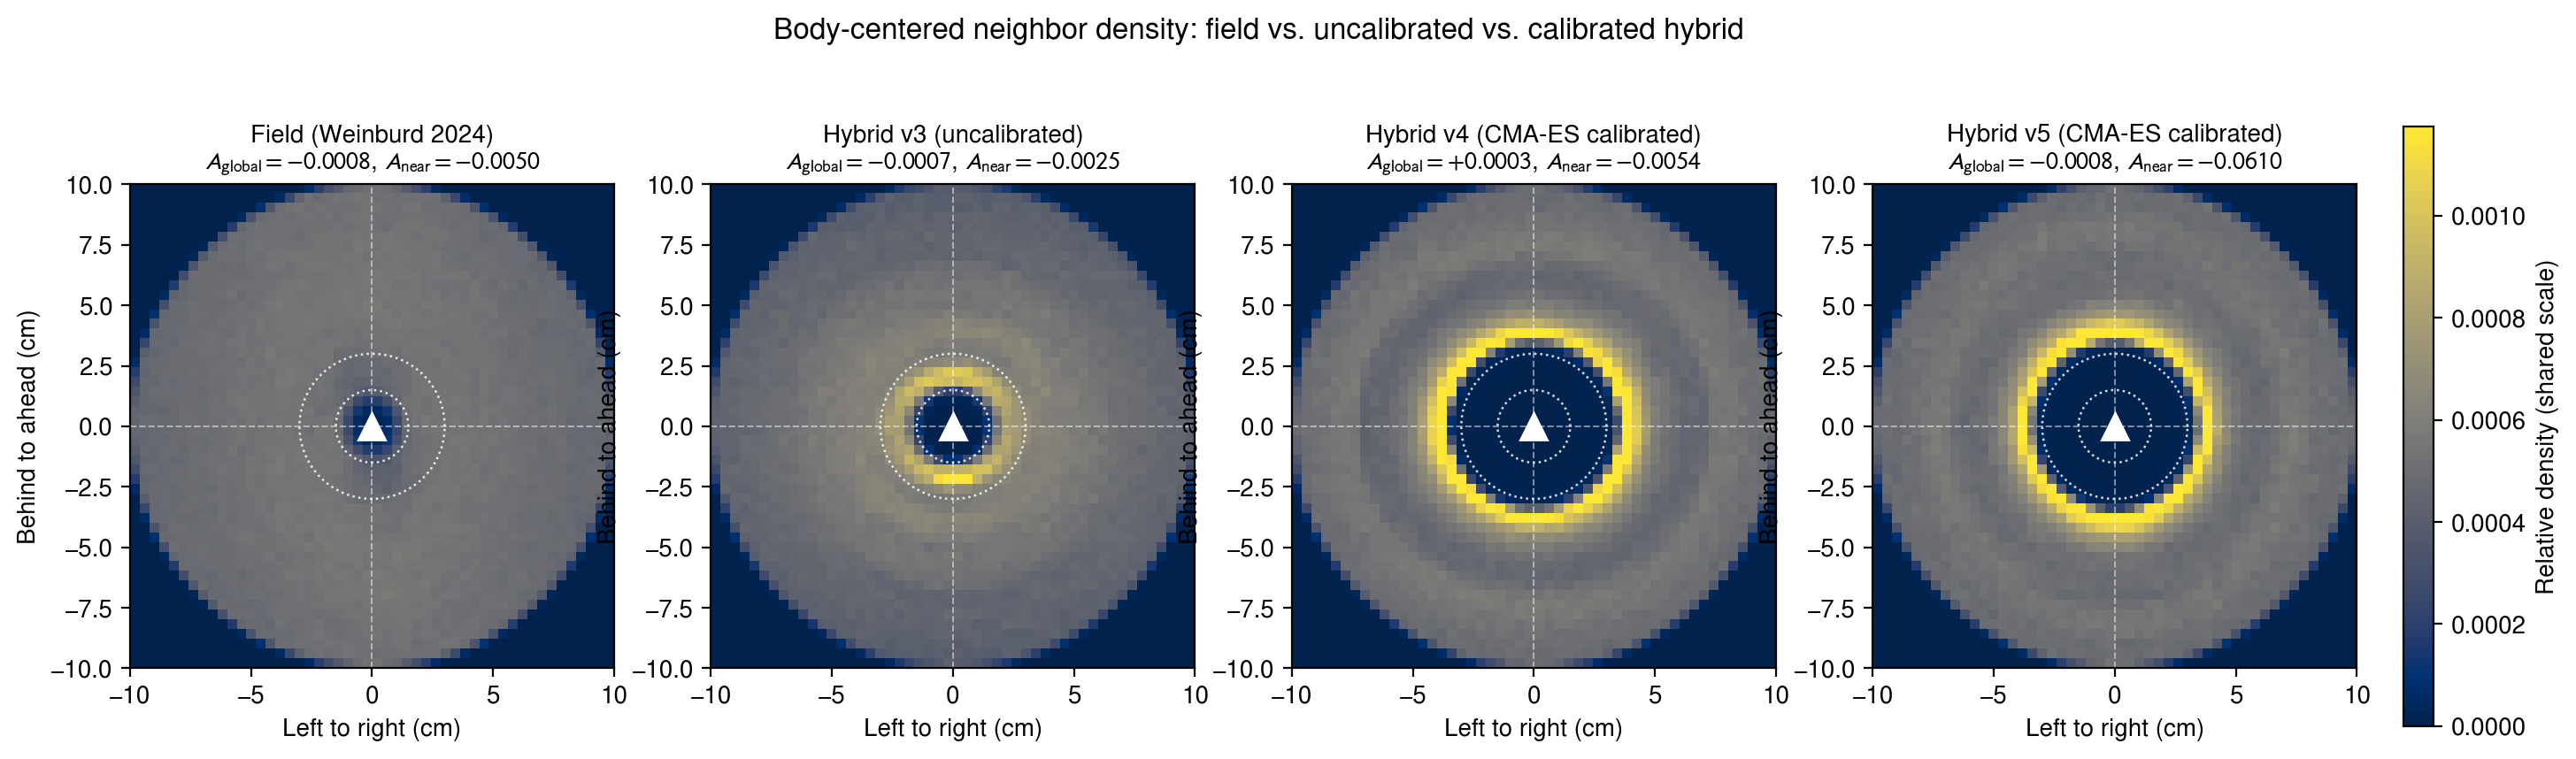
\includegraphics[width=\linewidth]{figures/fig4_spatial_check.png}
\caption{Body-centered neighbor density for the field and the three
hybrid models, on a shared color scale. The global anisotropy index
is within $|A| < 0.001$ of zero in all four. The near-zone index,
computed only inside the white dotted band ([1.5, 3.0]\,cm),
separates the v5 ring artifact ($A_\text{near} = -0.061$) from the
near-flat field ($-0.005$), v3 ($-0.003$), and v4 ($-0.005$). v4
fits both scalar and near-zone metrics; v5 trades the spatial fit
for a marginally lower scalar loss.}
\label{fig:fig4}
\end{figure}

The CMA-ES loss did not include $A_\text{near}$, so the optimizer
could place near-zone structure anywhere that did not break the three
scalar metrics. v4 found a basin in which the preferred-spacing ring
sits symmetrically around the focal ($\alpha_\text{aniso} = 0.80$,
$\lambda = 0.52$). v5, with the extra $\rho_\text{temporal}$
dimension, found a different basin: $\alpha_\text{aniso}$ saturates at
$0.99$ and $\lambda$ drops to $0.17$, which sharpens the ring and
biases it forward. v5's scalar loss is 0.085 versus v4's 0.099, so the
optimizer prefers it; on the spatial metric the trade goes the other
way. The seventh parameter is unnecessary at the field's measurement
scale, as Section~\ref{sec:cma-closes} already noted, and now actively
worsens the spatial fit. v4 is the configuration that matches all
four metrics; v5 is a worse fit dressed up as a slightly better one.

The ``void emerges'' claim from earlier v3 figures was an
overinterpretation of a feature that is small in the field. v3
reproduces the field's near-zone structure for the same reason it
fails the scalar metrics: forward-weighted alignment alone is enough
for spatial structure but not for tight heading control or NND.

\subsection{Boundary-condition dependence}

We tested the calibrated v4 model under reflective walls instead of
periodic boundaries. The fit broke: turning-angle std jumped to
0.493\,rad (78\% off) and NND dropped to 3.47\,cm (11\% off).
Polarization actually moved closer to target, from 0.898 to 0.752
(8.3\% off). The periodic image structure is doing real physical work
in the calibration. Reflective walls perturb headings on contact,
inflating the per-step turning distribution, and they compress
densities away from the boundary, lowering NND.

This matters because hopper bands are open systems with front and rear
asymmetry, not periodic boxes. A model intended to claim something
about field hopper-band dynamics needs to be calibrated under realistic
boundaries from the start, not validated against them after the fact.
We flag this as a limitation rather than a fix.

\section{Discussion}

We spent several weeks hand-tuning a hybrid model and producing scorecards
that captured one metric well at a time. CMA-ES, with parallel evaluation
across cores, runs end-to-end in about 13 minutes and finds parameter
combinations that hand-tuning missed. For noisy black-box objectives in
this dimensionality, derivative-free evolutionary search is the right
default. We should have used it sooner.

Adding temporal bearing integration ($\rho_\text{temporal}$) gave the
optimizer a seventh degree of freedom that it drove to its no-effect
limit ($\rho = 0.95$). On the scalar loss alone the change looks
benign and even slightly helpful, but the extra dimension also
shifted the converged basin: $\alpha_\text{aniso}$ saturated at $1.0$
in v5, against v4's $0.80$, and that re-shaped the preferred-spacing
ring into the forward-biased configuration that breaks the near-zone
fit (Section~\ref{sec:spatial}). The mechanism is not wrong in
principle, but at the field's measurement scale it is unnecessary and,
in our calibration, harmful. Future work that tests
\citet{sayin2025}'s ring-attractor proposal will need a measurement
that distinguishes instantaneous from time-integrated bearing
estimation, which neither our scalar nor our spatial metrics do.

The remaining gap is polarization. The v4 and v5 calibrations sit at
$\Phi \approx 0.89$ versus a field target of $0.82$. We re-ran v4 with
equal weights ($w_\Phi = w_\sigma = w_\text{NND} = 1$) to test whether
the gap was an artifact of our prioritized weighting. The equal-weight
optimum lands at $\Phi = 0.883$, $\sigma = 0.277$\,rad, NND
$= 3.92$\,cm, with $\lambda$ dropping from $0.52$ to $0.24$ and
$\alpha_\text{aniso}$ saturating at $0.99$. The polarization gap
narrows by 0.015 and the other two metrics do not break. v4's
polarization floor is therefore close to $0.88$ regardless of
weighting, which we read as a structural property of the model at
this density rather than a tunable parameter.

We have not run an open-boundary calibration. The reflective-wall
stress test indicates the trade-offs differ. Three plausible follow-ups
are: a flux-boundary scheme that despawns leaving agents and respawns
at the rear; calibration under reflective walls with the loss reweighted;
or a sliding-window simulation centered on the swarm centroid. We did
not have time to implement any of these.

\section{Project contributions}

\textbf{Asher Albrecht} built the field-data ingestion pipeline from the
\citet{weinburd2024} \texttt{.mat} files, computed the four baseline
metrics on the field data (Section 3.1), implemented the Vicsek and Pull
baseline models, and led the hybrid v3 anisotropic-Vicsek design and the
$\eta$/$\lambda$ parameter sweep figures.

\textbf{George Stephenson} extended the hybrid model with heading inertia,
preferred spacing, and temporal bearing integration (v4 and v5 in
\texttt{hybrid\_v4.py} and \texttt{hybrid\_v5.py}), built the parallel
CMA-ES calibration framework (\texttt{calibrate\_cma.py},
\texttt{calibrate\_cma\_v5.py}, \texttt{validate\_calibrated.py}),
implemented the spatial-anisotropy validation against the field density
map, and produced the post-calibration figures.

Both authors contributed to the experimental design, the slide deck,
and this paper.

\section*{Code and data}

The simulation code, calibration scripts, CMA-ES log files, and figure
generators are at \url{https://github.com/}\textit{(repo to be added on
submission)}. The Weinburd dataset is available from the original
authors at \citet{weinburd2024}.

\bibliographystyle{plainnat}
\bibliography{refs}

\end{document}
